% Converted from reference/DB4OFlare (MadCap Flare, Java target)

\chapter{Platform Specific Issues}
\label{ref:platform-specific-issues}

Db4o can be run in a variety of environments, which have Java virtual machine or .NET CLR. We use a common core code base, which allows automatic production of db4o builds for the following platforms:

\begin{itemize}
\item Java JDK 5 or newer
\item .NET 3.5 or newer
\item .NET 3.5 CompactFramework
\item Mono (you need to compile db4o yourself)
\item Android
\item Silverlight
\end{itemize}

Db4o has a small database footprint and requires minimum processing resources thus being an excellent choice for embedded use in smartphones, photocopiers, car electronics, and packaged software (including real-time monitoring systems). It also shows good performance and reliability in web and desktop applications.

You can use db4o on desktop with:

\begin{itemize}
\item Windows (Java, .Net)
\item Linux (Java, Mono).
\end{itemize}

On mobile and embedded devices with:

\begin{itemize}
\item Android
\item Windows CE or Windows Mobile (.NET Compact Framework)
\end{itemize}

db4o provides the same API for all platforms, however each platform has its own features, which should be taken into consideration in software development process. These features will be discussed in the following chapters.

More Reading:

\begin{itemize}
\item \hyperref[ref:platform-specific-issues-db4o-on-java-platforms]{db4o on Java Platforms} (p.~\pageref{ref:platform-specific-issues-db4o-on-java-platforms})
\item \hyperref[ref:platform-specific-issues-security-requirements-on-java-platform]{Security Requirements On Java Platform} (p.~\pageref{ref:platform-specific-issues-security-requirements-on-java-platform})
\item \hyperref[ref:platform-specific-issues-web-servlets]{Servlets} (p.~\pageref{ref:platform-specific-issues-web-servlets})
\item \hyperref[ref:platform-specific-issues-database-for-osgi]{Database For OSGi} (p.~\pageref{ref:platform-specific-issues-database-for-osgi})
\item \hyperref[ref:platform-specific-issues-android]{Android} (p.~\pageref{ref:platform-specific-issues-android})
\end{itemize}

\section{Disconnected Objects}
\label{ref:platform-specific-issues-disconnected-objects}

db4o manages objects \hyperref[ref:basics-identity-concept]{by object-identity} (p.~\pageref{ref:basics-identity-concept}). db4o ensures that each stored object in the database is always represented by the same object in memory. When you load an object, change it and then store it, db4o recognizes the object by its identity and will update it.

This model works wonderful as long as the object-identity is preserved. However there are a lot of scenarios, where the object-identity is lost. As soon as serialize objects, the object-identity is lost. This is typical for web-scenarios or web-services, where a object needs to be identified across requests. For such scenarios objects need additional ids to identify object across requests- and object-container-boundaries.

There are several possibilities for such additional ids. You can use db4o internal ids, \hyperref[ref:advanced-topics-ids-and-uuids]{db4o uuids} (p.~\pageref{ref:advanced-topics-ids-and-uuids}), or additional ids-fields on objects. Each has its advantages and disadvantages, so take a looks at this comparison: \hyperref[ref:platform-specific-issues-disconnected-objects-comparison-of-ids]{See "Comparison Of Different IDs"} (p.~\pageref{ref:platform-specific-issues-disconnected-objects-comparison-of-ids})

Only identifying the object across object container boundaries is often not enough. You actually need to update a disconnected object. This is done by coping the new values to the existing object. \hyperref[ref:platform-specific-issues-disconnected-objects-merging-changes]{See "Merging Changes"} (p.~\pageref{ref:platform-specific-issues-disconnected-objects-merging-changes})

\subsection{Comparison Of Different IDs}
\label{ref:platform-specific-issues-disconnected-objects-comparison-of-ids}

There are a lot of possibilities for additional ids to identify objects across the object container boundary.

\subsubsection*{Internal db4o ids}

db4o has internal ids to identify each object in the database. You can access these ids and use them yourself. . Take a look at the example. \hyperref[ref:platform-specific-issues-disconnected-objects-example-internal-id]{See "Example Internal Id"} (p.~\pageref{ref:platform-specific-issues-disconnected-objects-example-internal-id})

{\small
\begin{longtable}{|p{\dimexpr(\linewidth-3\arrayrulewidth)*1/2-2\tabcolsep\relax}|p{\dimexpr(\linewidth-3\arrayrulewidth)*1/2-2\tabcolsep\relax}|}
\hline
\textbf{Advantages} & \textbf{Disadvantages} \\ \hline
\begin{itemize}
\item Internal ids are fast.
\item No additional field on the class required.
\item No additional configuration required.
\end{itemize} & \begin{itemize}
\item The id may change when defragmentating the database.
\end{itemize} \\ \hline
\end{longtable}}

\subsubsection*{db4o UUIDs}

db4o supports special UUIDs. You can enable them by configuration. . Take a look at the example. \hyperref[ref:platform-specific-issues-disconnected-objects-example-db4o-uuid]{See "Example db4o UUID"} (p.~\pageref{ref:platform-specific-issues-disconnected-objects-example-db4o-uuid})

{\small
\begin{longtable}{|p{\dimexpr(\linewidth-3\arrayrulewidth)*1/2-2\tabcolsep\relax}|p{\dimexpr(\linewidth-3\arrayrulewidth)*1/2-2\tabcolsep\relax}|}
\hline
\textbf{Advantages} & \textbf{Disadvantages} \\ \hline
\begin{itemize}
\item A UUID is a worldwide unique id.
\item No additional field on the class required.
\end{itemize} & \begin{itemize}
\item db4o UUIDs are large.
\item db4o UUID is db4o-specific type.
\end{itemize} \\ \hline
\end{longtable}}

\subsubsection*{UUID-Fields on Classes}

You can add UUID-fields to your classes. In the constructor of the object you assign a new UUID to the object. Then you can find the object by a regular query. Add \hyperref[ref:advanced-topics-type-handling-uuid-support]{UUID support} (p.~\pageref{ref:advanced-topics-type-handling-uuid-support}) before using UUIDs . Don't forget \hyperref[ref:basics-indexing]{to index the id-field} (p.~\pageref{ref:basics-indexing}). Take a look at the example. \hyperref[ref:platform-specific-issues-disconnected-objects-example-plattform-uuid]{See "Example "} (p.~\pageref{ref:platform-specific-issues-disconnected-objects-example-plattform-uuid})

{\small
\begin{longtable}{|p{\dimexpr(\linewidth-3\arrayrulewidth)*1/2-2\tabcolsep\relax}|p{\dimexpr(\linewidth-3\arrayrulewidth)*1/2-2\tabcolsep\relax}|}
\hline
\textbf{Advantages} & \textbf{Disadvantages} \\ \hline
\begin{itemize}
\item A UUID is a worldwide unique id .
\item UUID are easy to generate and portable.
\end{itemize} & \begin{itemize}
\item You need an id-field on your objects.
\item UUIDs are quite large.
\item Additional index required.
\end{itemize} \\ \hline
\end{longtable}}

\subsubsection*{ID-Field On Classes With a ID-Generator}

You can add a id-field to your classes and then use an ID-Generator to assign new ids to stored objects. Don't forget \hyperref[ref:basics-indexing]{to index the id-field} (p.~\pageref{ref:basics-indexing}). Take a look at the example. \hyperref[ref:platform-specific-issues-disconnected-objects-example-id-generator]{See "Example ID-Generator"} (p.~\pageref{ref:platform-specific-issues-disconnected-objects-example-id-generator})

{\small
\begin{longtable}{|p{\dimexpr(\linewidth-3\arrayrulewidth)*1/2-2\tabcolsep\relax}|p{\dimexpr(\linewidth-3\arrayrulewidth)*1/2-2\tabcolsep\relax}|}
\hline
\textbf{Advantages} & \textbf{Disadvantages} \\ \hline
\begin{itemize}
\item A simple id on objects.
\item Familiar model from the RDBMS-world.
\end{itemize} & \begin{itemize}
\item You need an id-field on your objects.
\item You need to implement an ID-Generator. Which isn't trivial.
\item Additional index required.
\end{itemize} \\ \hline
\end{longtable}}

\subsubsection{Example Internal Id}
\label{ref:platform-specific-issues-disconnected-objects-example-internal-id}

This example demonstrates how you can use internal object ids to identify objects across objects containers. Take a look advantages and disadvantages of internal ids: \hyperref[ref:platform-specific-issues-disconnected-objects-comparison-of-ids]{See "Comparison Of Different IDs"} (p.~\pageref{ref:platform-specific-issues-disconnected-objects-comparison-of-ids})

For using the internal ids no additional configuration is required. You can get this id for any object.

You can get the internal id from the extended object container.

\begin{lstlisting}
long interalId = container.ext().getID(obj);
\end{lstlisting}

{\small\itshape Db4oInternalIdExample.java: get the db4o internal ids\par}
\medskip

Getting a object by its id is also easy. First you get the object from the container. Unlike queries this won't return a \hyperref[ref:basics-activation]{activated} (p.~\pageref{ref:basics-activation}) object. So you have to do it explicitly.

\begin{lstlisting}
long internalId =idForObject;
Object objectForID = container.ext().getByID(internalId);
// getting by id doesn't activate the object
// so you need to do it manually
container.ext().activate(objectForID);
\end{lstlisting}

{\small\itshape Db4oInternalIdExample.java: get an object by db4o internal id\par}
\medskip

\subsubsection{Example db4o UUID}
\label{ref:platform-specific-issues-disconnected-objects-example-db4o-uuid}

This example demonstrates how you can use db4o-UUIDs to identify objects across objects containers. Take a look advantages and disadvantages of db4o-UUIDs: \hyperref[ref:platform-specific-issues-disconnected-objects-comparison-of-ids]{See "Comparison Of Different IDs"} (p.~\pageref{ref:platform-specific-issues-disconnected-objects-comparison-of-ids})

First you need to enable db4o-UUIDs in order to use it.

\begin{lstlisting}
configuration.file().generateUUIDs(ConfigScope.GLOBALLY);
\end{lstlisting}

{\small\itshape Db4oUuidExample.java: db4o-uuids need to be activated\par}
\medskip

With UUIDs turned on, db4o will create an UUID for each stored object. So you can get the UUID of the object from the object-container.

\begin{lstlisting}
Db4oUUID uuid = container.ext().getObjectInfo(obj).getUUID();
\end{lstlisting}

{\small\itshape Db4oUuidExample.java: get the db4o-uuid\par}
\medskip

Getting a object by its UUID is also easy. First you get the object from the container. Unlike queries this won't \hyperref[ref:basics-activation]{activate} (p.~\pageref{ref:basics-activation}) your object. So you have to do it explicitly.

\begin{lstlisting}
Object objectForId = container.ext().getByUUID(idForObject);
// getting by uuid doesn't activate the object
// so you need to do it manually
container.ext().activate(objectForId);
\end{lstlisting}

{\small\itshape Db4oUuidExample.java: get an object by a db4o-uuid\par}
\medskip

\subsubsection{Example UUID}
\label{ref:platform-specific-issues-disconnected-objects-example-plattform-uuid}

This example demonstrates how you can use UUID s to identify objects across objects containers. Take a look advantages and disadvantages of UUID s: \hyperref[ref:platform-specific-issues-disconnected-objects-comparison-of-ids]{See "Comparison Of Different IDs"} (p.~\pageref{ref:platform-specific-issues-disconnected-objects-comparison-of-ids})

Don't forget to add \hyperref[ref:advanced-topics-type-handling-uuid-support]{UUID support} (p.~\pageref{ref:advanced-topics-type-handling-uuid-support}).

This example assumes that all object have a common super class, IDHolder, which holds the UUID in a field.

\begin{lstlisting}
private final UUID uuid = UUID.randomUUID();

public UUID getObjectId(){
    return uuid;
}
\end{lstlisting}

{\small\itshape IDHolder.java: generate the id\par}
\medskip

It's important to index the id-field, otherwise looking up for object by id will be slow.

\begin{lstlisting}
configuration.common().add(new UuidSupport());
configuration.common().objectClass(IDHolder.class).objectField("uuid").indexed(true);
\end{lstlisting}

{\small\itshape UuidOnObject.java: index the uuid-field\par}
\medskip

The id is hold by the object itself, so you can get it directly.

\begin{lstlisting}
IDHolder uuidHolder = (IDHolder)obj;
UUID uuid = uuidHolder.getObjectId();
\end{lstlisting}

{\small\itshape UuidOnObject.java: get the uuid\par}
\medskip

You can get the object you can by a regular query.

\begin{lstlisting}
Query query = container.query();
query.constrain(IDHolder.class);
query.descend("uuid").constrain(idForObject);
IDHolder object= (IDHolder) query.execute().get(0);
\end{lstlisting}

{\small\itshape UuidOnObject.java: get an object its UUID\par}
\medskip

\subsubsection{Example ID-Generator}
\label{ref:platform-specific-issues-disconnected-objects-example-id-generator}

This example demonstrates how you can use an ID-generator to identify objects across objects containers. Take a look advantages and disadvantages of ID-generators: \hyperref[ref:platform-specific-issues-disconnected-objects-comparison-of-ids]{See "Comparison Of Different IDs"} (p.~\pageref{ref:platform-specific-issues-disconnected-objects-comparison-of-ids})

This example assumes that all object have a common super class, IDHolder, which holds the id.

\begin{lstlisting}
private int id;
public int getId() {
    return id;
}

public void setId(int id) {
    this.id = id;
}
\end{lstlisting}

{\small\itshape IDHolder.java: id holder\par}
\medskip

Don't forget to index the id-field. Otherwise finding objects by id will be slow.

\begin{lstlisting}
configuration.common().objectClass(IDHolder.class).objectField("id").indexed(true);
\end{lstlisting}

{\small\itshape AutoIncrementExample.java: index the id-field\par}
\medskip

The hard part is to write an efficient ID-Generator. For this example a very simple \hyperref[ref:advanced-topics-callbacks-possible-usecases-autoincrement]{auto increment generator} (p.~\pageref{ref:advanced-topics-callbacks-possible-usecases-autoincrement}) is used. Use the \hyperref[ref:advanced-topics-callbacks-event-registry-api]{creating-callback-event} (p.~\pageref{ref:advanced-topics-callbacks-event-registry-api}) in order to add the ids to the object. When committing, store the state of the id-generator.

\begin{lstlisting}
final AutoIncrement increment = new AutoIncrement(container);
EventRegistry eventRegistry = EventRegistryFactory.forObjectContainer(container);
eventRegistry.creating().addListener(new EventListener4<CancellableObjectEventArgs>() {
    public void onEvent(Event4<CancellableObjectEventArgs> event4,
                        CancellableObjectEventArgs objectArgs) {
        if(objectArgs.object() instanceof IDHolder){
            IDHolder idHolder = (IDHolder) objectArgs.object();
            idHolder.setId(increment.getNextID(idHolder.getClass()));
        }
    }
});
eventRegistry.committing().addListener(new EventListener4<CommitEventArgs>() {
    public void onEvent(Event4<CommitEventArgs> commitEventArgsEvent4,
                        CommitEventArgs commitEventArgs) {
        increment.storeState();
    }
});
\end{lstlisting}

{\small\itshape AutoIncrementExample.java: use events to assign the ids\par}
\medskip

The id is hold by the object itself, so you can get it directly.

\begin{lstlisting}
IDHolder idHolder = (IDHolder)obj;
int id = idHolder.getId();
\end{lstlisting}

{\small\itshape AutoIncrementExample.java: get the id\par}
\medskip

You can get the object you can by a regular query.

\begin{lstlisting}
Object object = container.query(new Predicate<IDHolder>() {
    @Override
    public boolean match(IDHolder o) {
        return o.getId() == id;
    }
}).get(0);
\end{lstlisting}

{\small\itshape AutoIncrementExample.java: get an object by its id\par}
\medskip

\subsection{Merging Changes}
\label{ref:platform-specific-issues-disconnected-objects-merging-changes}

Merging the changes is the most challenging part when using disconnected objects. Imagine that we have a disconnected object, which contains the changes. We have to store the changes somehow. You cannot simply store the disconnected object, because db4o wouldn't recognize it and store a new object instead of updating the old one. \hyperref[ref:platform-specific-issues-disconnected-objects-wrong-approach]{See "Wrong Approach"} (p.~\pageref{ref:platform-specific-issues-disconnected-objects-wrong-approach})

Instead you need to load the existing object and then copy the state from the disconnected object to the loaded object. Basically you traverse the object-graph and copy all changes over. \hyperref[ref:platform-specific-issues-disconnected-objects-example-merge-changes]{See "Example Merge Changes"} (p.~\pageref{ref:platform-specific-issues-disconnected-objects-example-merge-changes})

db4o has no built-in merge support. However there are external libraries which can help you to merge changes, like  \href{http://dozer.sourceforge.net/}{Dozer}.

\subsubsection{Wrong Approach}
\label{ref:platform-specific-issues-disconnected-objects-wrong-approach}

The wrong approach is to try to store disconnected objects. db4o manages object by their \hyperref[ref:basics-identity-concept]{object-identity} (p.~\pageref{ref:basics-identity-concept}) and doesn't recognize objects which have been serialized or loaded by another object container instance. This example shows, that instead of updating the object, db4o will store a new instance of the object.

\begin{lstlisting}
{
    ObjectContainer container = openDatabase();
    Pilot joe = queryByName(container,"Joe");
    container.close();

    // The update on another object container
    ObjectContainer otherContainer = openDatabase();
    joe.setName("Joe New");
    otherContainer.store(joe);
    otherContainer.close();
}
{
    // instead of updating the existing pilot,
    // a new instance was stored.
    ObjectContainer container = openDatabase();
    ObjectSet<Pilot> pilots = container.query(Pilot.class);
    System.out.println("Amount of pilots: "+pilots.size());
    for (Pilot pilot : pilots) {
        System.out.println(pilot);
    }
    container.close();
}
\end{lstlisting}

{\small\itshape ObjectIdentityExamples.java: Update doesn't works when using the different object containers\par}
\medskip

So in order to update an object, you need to load and store it in the same object-container. If you cannot do this, you need to merge to object-changes. \hyperref[ref:platform-specific-issues-disconnected-objects-example-merge-changes]{See "Example Merge Changes"} (p.~\pageref{ref:platform-specific-issues-disconnected-objects-example-merge-changes})

\begin{lstlisting}
{
    ObjectContainer container = openDatabase();
    Pilot joe = queryByName(container,"Joe");
    joe.setName("Joe New");
    container.store(joe);
    container.close();
}
{
    ObjectContainer container = openDatabase();
    ObjectSet<Pilot> pilots = container.query(Pilot.class);
    System.out.println("Amount of pilots: "+pilots.size());
    for (Pilot pilot : pilots) {
        System.out.println(pilot);
    }
    container.close();
}
\end{lstlisting}

{\small\itshape ObjectIdentityExamples.java: Update works when using the same object container\par}
\medskip

\subsubsection{Example Merge Changes}
\label{ref:platform-specific-issues-disconnected-objects-example-merge-changes}

This example shows how changes are merged from the disconnected object to the object to update. To do this, traverse the object-graph and copy all value types over. All reference types are first checked if they are an existing object. If it is,the primitives are copied over, otherwise it's a stored as a new object.

\begin{lstlisting}
ObjectContainer container = openDatabase();

// first get the object from the database
Car carInDb = getCarById(container,disconnectedCar.getObjectId());

// copy the value-objects (int, long, double, string etc)
carInDb.setName(disconnectedCar.getName());

// traverse into the references
Pilot pilotInDB = carInDb.getPilot();
Pilot disconnectedPilot = disconnectedCar.getPilot();

// check if the object is still the same
if(pilotInDB.getObjectId().equals(disconnectedPilot.getObjectId())){
    // if it is, copy the value-objects
    pilotInDB.setName(disconnectedPilot.getName());
    pilotInDB.setPoints(disconnectedPilot.getPoints());
} else{
    // otherwise replace the object
    carInDb.setPilot(disconnectedPilot); 
}

// finally store the changes
container.store(pilotInDB);
container.store(carInDb);
\end{lstlisting}

{\small\itshape MergeExample.java: merging\par}
\medskip

You can use reflection to automated this process. You can also use existing libraries like  \href{http://dozer.sourceforge.net/}{Dozer} which help you to do this.

\section{Web Environment}
\label{ref:platform-specific-issues-web-environment}

db4o runs perfectly well in a web environment. It can be used to build your web-application.

In most web-application multiple concurrent requests are processes. Normally you want to isolate each request from another. You can use db4o transactions to archive this isolation. \hyperref[ref:platform-specific-issues-web-web-isolation]{See "Isolation in Web-Applications".} (p.~\pageref{ref:platform-specific-issues-web-web-isolation})

In most web-applications a object is only alive during a request. So you have to identify objects across requests. Therefore you need to add an additional id to your object. There are different possibilities for this. \hyperref[ref:platform-specific-issues-disconnected-objects]{See "Disconnected Objects"} (p.~\pageref{ref:platform-specific-issues-disconnected-objects})

When you run in a web-environment, you often have stricter security limitations. Take a look at the security requirements. \hyperref[ref:platform-specific-issues-security-requirements-on-java-platform]{See "Security Requirements"} (p.~\pageref{ref:platform-specific-issues-security-requirements-on-java-platform})

Take a look how you create a object-container for each request. \hyperref[ref:platform-specific-issues-web-servlets]{See "Servlets"} (p.~\pageref{ref:platform-specific-issues-web-servlets})

Take a look at a small example Spring MVC application.\hyperref[ref:platform-specific-issues-web-spring-mvc-example]{See "Spring MVC Example"} (p.~\pageref{ref:platform-specific-issues-web-spring-mvc-example})

\subsection{Isolation in Web-Applications}
\label{ref:platform-specific-issues-web-web-isolation}

In most web-application multiple concurrent request are processes. You want to isolate the request from each other. db4o supports \hyperref[ref:basics-acid-and-transactions]{transactions} (p.~\pageref{ref:basics-acid-and-transactions}), which are perfect for this kind of isolation. Each unit of work gets its own transaction, for example each request. You can create a new session object container for this purpose. Such a session-container brings its own transaction and reference-system. This ensures that the session container is isolated from other operations on the database.

\begin{lstlisting}
ObjectContainer rootContainer = Db4oEmbedded.openFile(DATABASE_FILE_NAME);

// open the db4o-session. For example at the beginning for a web-request
ObjectContainer session = rootContainer.ext().openSession();
try {
    // do the operations on the session-container
    session.store(new Person("Joe"));
} finally {
    // close the container. For example when the request ends
    session.close();
}
\end{lstlisting}

{\small\itshape Db4oSessions.java: Session object container\par}
\medskip

Or you can use embedded clients when your \hyperref[ref:client-server-embedded]{embedded clients} (p.~\pageref{ref:client-server-embedded}).

\begin{lstlisting}
ObjectServer server = Db4oClientServer.openServer(DATABASE_FILE_NAME, 0);

// open the db4o-embedded client. For example at the beginning for a web-request
ObjectContainer container = server.openClient();
try {
    // do the operations on the session-container
    container.store(new Person("Joe"));
} finally {
    // close the container. For example when the request ends
    container.close();
}
\end{lstlisting}

{\small\itshape Db4oSessions.java: Embedded client\par}
\medskip

\subsection{Servlets}
\label{ref:platform-specific-issues-web-servlets}

Running db4o as the persistence layer of a Java web application is easy. There is no installation procedure - db4o is just another library in your application. There are only two issues that make web applications distinct from standalone programs from db4o's point of view. One is the more complex classloader environment - db4o needs to know itself and the classes to be persisted.

The other issue is configuring, starting and shutting down the db4o correctly. This can be done at the Servlet API layer or within the web application framework you are using.

On the Servlet API layer, you could bind db4o server handling to the Servlet.

You can implement the ServletContextListener-interface, open the database when the web application starts and close when it ends.

\begin{lstlisting}
@Override
public void contextInitialized(ServletContextEvent event) {
    ServletContext context = event.getServletContext();
    String filePath = context.getRealPath("WEB-INF/"
            + context.getInitParameter(KEY_DB4O_FILE_NAME));
    EmbeddedObjectContainer rootContainer = Db4oEmbedded.openFile(filePath);
    context.setAttribute(KEY_DB4O_SERVER, rootContainer);
    context.log("db4o startup on " + filePath);
}

@Override
public void contextDestroyed(ServletContextEvent event) {
    ServletContext context = event.getServletContext();
    ObjectContainer rootContainer = (ObjectContainer) context.getAttribute(KEY_DB4O_SERVER);
    context.removeAttribute(KEY_DB4O_SERVER);
    close(rootContainer);
    context.log("db4o shutdown");
}
\end{lstlisting}

{\small\itshape Db4oServletListener.java: db4o-instance for the web-application\par}
\medskip

Additionally you can implement the ServletRequestListener-interface and open a \hyperref[ref:platform-specific-issues-web-web-isolation]{db4o-session} (p.~\pageref{ref:platform-specific-issues-web-web-isolation}) on each request.

\begin{lstlisting}
@Override
public void requestInitialized(ServletRequestEvent requestEvent) {
    EmbeddedObjectContainer rootContainer = (EmbeddedObjectContainer) requestEvent
            .getServletContext().getAttribute(Db4oServletListener.KEY_DB4O_SERVER);

    ObjectContainer session = rootContainer.openSession();
    requestEvent.getServletRequest().setAttribute(KEY_DB4O_SESSION, session);
}

@Override
public void requestDestroyed(ServletRequestEvent requestEvent) {
    ObjectContainer session = (ObjectContainer) requestEvent
            .getServletRequest().getAttribute(KEY_DB4O_SESSION);

    close(session);
}
\end{lstlisting}

{\small\itshape Db4oServletListener.java: a db4o-session for each request\par}
\medskip

This listener has to be registered in the web.xml.

\begin{lstlisting}
<context-param>
    <param-name>database-file-name</param-name>
    <param-value>database.db4o</param-value>
</context-param>
<listener>
    <listener-class>com.db4odoc.servlet.Db4oServletListener</listener-class>
</listener>
\end{lstlisting}

{\small\itshape web.xml: register the listener for the web application\par}
\medskip

Now db4o should be available to your application classes. Each request has it own object-container. You can get the instance via its key, like this:

\begin{lstlisting}
ObjectContainer container = 
        (ObjectContainer)req.getAttribute(Db4oServletListener.KEY_DB4O_SESSION);
\end{lstlisting}

{\small\itshape ServletExample.java: Get the session container\par}
\medskip

However, We strongly suggest that you use the features provided by your framework and that you consider not exposing db4o directly to your application logic. (There is nothing db4o-specific about these recommendentations, we would vote for this in the presence of any persistence layer.)

\subsection{Spring MVC Example}
\label{ref:platform-specific-issues-web-spring-mvc-example}

This example is a tiny CRUD application which shows how to use db4o in a web-application. This example uses the \href{http://www.springsource.org/}{Spring MVC} framework. Of course, db4o works with any webframework.

\subsubsection*{Managing Object Containers}

It uses the code from the \hyperref[ref:platform-specific-issues-web-servlets]{servlet-example} (p.~\pageref{ref:platform-specific-issues-web-servlets}) to have a object container for each request. On each new request a object container is opened. Then all operations are done on the container. When the request ends, the container is closed.

You also can use the features of your web framework or your dependency injection framework to archive the same goal.

\subsubsection*{Object Identification}

This example uses a GUID for each object to identify it across requests. Persisted objects which inherit from the IDHolder class which contains the id-field. Take a look at alternatives for ids. \hyperref[ref:platform-specific-issues-disconnected-objects-comparison-of-ids]{See "Comparison Of Different IDs"} (p.~\pageref{ref:platform-specific-issues-disconnected-objects-comparison-of-ids})

\subsubsection*{Using db4o}

You can use db4o as expected. In this example we use a the db4o-container of the request:

\begin{lstlisting}
@RequestMapping(value = "list.html", method = RequestMethod.GET)
public ModelAndView get() {
    ObjectSet pilots = db4o.objectContainer().query(Pilot.class);
    return new ModelAndView("list", "pilots", new ArrayList<Pilot>(pilots));
}
\end{lstlisting}

{\small\itshape HomeController.java: List all pilots on the index-page\par}
\medskip

\subsubsection*{Using IDs}

Now the ids can be used in the views and controllers to identify objects. For example in a list-view you use the ids for the edit- and delete-links:

\begin{lstlisting}
<c:forEach items="${pilots}" var="pilot">
    <tr>
        <td>
            <a href="edit${pilot.id}.html"/>Edit</a>
            <a href="delete${pilot.id}.html"/>Delete</a>
        </td>
        <td>
                ${pilot.name}
        </td>
        <td>
                ${pilot.points}
        </td>
    </tr>
</c:forEach>
\end{lstlisting}

{\small\itshape list.jsp: In the view use the ids to identify the objects\par}
\medskip

Another location where the ids are used is in the controllers. For example when you need to store changes. First we get a object which contains all changes. Then we copy all changes to the existing object in the database and finally store it. \hyperref[ref:platform-specific-issues-disconnected-objects-merging-changes]{See "Merging Changes"} (p.~\pageref{ref:platform-specific-issues-disconnected-objects-merging-changes})

\begin{lstlisting}
@RequestMapping(value = "/edit{id}.html", method = RequestMethod.POST)
public ModelAndView editPilot(@PathVariable final String id, Pilot pilotFromForm) {
    Pilot pilotFromDatabase = db4o.objectContainer().query(new Predicate<Pilot>() {
        @Override
        public boolean match(Pilot p) {
            return p.getId().equals(id);
        }
    }).get(0);
    pilotFromDatabase.setName(pilotFromForm.getName());
    pilotFromDatabase.setPoints(pilotFromForm.getPoints());
    db4o.objectContainer().store(pilotFromDatabase);
    return new ModelAndView(new RedirectView("list.html"));
}
\end{lstlisting}

{\small\itshape HomeController.java: Update the object\par}
\medskip

\section{Reporting}
\label{ref:platform-specific-issues-reporting}

You want to generate reports with from a db4o database? What capabilities does db4o have to support reporting? How can you implement reporting? This topic tries to answer these questions.

\subsection*{Understand db4o's Limitations}

db4o has serious limitations when it comes to reporting. It doesn't support any aggregation operations like average, min, max or sum. Nor does it support any projection (SELECT statement in SQL) or grouping operations. You only can query for objects and not do any statistics or selection on them.

\subsection*{Reporting with db4o}

Despite the missing features for reporting it's possible to do simple reports with db4o as long as your reporting framework can work with simple Java Beans instead of a relational database. Take a look at this small example with Jasper Reports. \hyperref[ref:platform-specific-issues-reporting-db4o-with-jasper]{See "db4o with Jasper Reports Example"} (p.~\pageref{ref:platform-specific-issues-reporting-db4o-with-jasper})

\subsection*{Separate Application Data from Reporting Data}

In some applications it can make sense to separate application data from the reporting data, for e example in a web application. The visits log data goes into a relational database which then is used for reporting, while the content of the site is stored in db4o. In this case you the can use the full power of the relational database for the reporting of the visitor data.

\subsection*{Export to a Relation Database}

Another possibility would be to export the data to a relational database for reporting purposes. In that process you also can denormalize and restructure the data for the reporting task. That way you also can use a regular relational database for the reporting tasks.

\subsection{db4o with Jasper Reports Example}
\label{ref:platform-specific-issues-reporting-db4o-with-jasper}

This example illustrates how you can use Jasper Reports together with db4o to create a report. Take a look at the official \href{http://jasperforge.org/}{Jasper Reports website} for the documentation and tools around Jasper Reports.

\subsubsection*{Designing the Report}

The report layout is written as an XML file or alternatively you can use an editor like the \href{http://jasperforge.org/projects/ireport}{iReport}-editor.

For adding data you can declare fields, which then are used for each row of the report. Just use the names of your properties which you want to report. For navigating along the data separate the properties with dots:

\begin{lstlisting}
<field name="sirname" class="java.lang.String"/>
<field name="firstname" class="java.lang.String"/>
<field name="address.city" class="java.lang.String"/>
\end{lstlisting}

{\small\itshape report.jrxml: declare fields\par}
\medskip

After that you can access these fields in the report:

\begin{lstlisting}
<textField>
    <reportElement x="0" y="0" width="100" height="21"/>
    <textFieldExpression class="java.lang.String"><![CDATA[$F{sirname}]]></textFieldExpression>
</textField>
<textField>
    <reportElement x="100" y="0" width="100" height="21"/>
    <textFieldExpression class="java.lang.String"><![CDATA[$F{firstname}]]></textFieldExpression>
</textField>
<textField>
    <reportElement x="200" y="0" width="100" height="21"/>
    <textFieldExpression class="java.lang.String"><![CDATA[$F{address.city}]]></textFieldExpression>
</textField>
\end{lstlisting}

{\small\itshape report.jrxml: Placing the fields on the report\par}
\medskip

\subsubsection*{Filling the Report}

After that you can fill the report with data from the database. For simpler reports we can use the JRBeanCollectionDataSource, which reads the values from regular Java bean objects. For more complex reports you might need to use another data source which you can fill manually like the JRMapCollectionDataSource. For all the available datasources read the \href{http://jasperforge.org/website/jasperreportswebsite/trunk/documentation.html}{Jasper Reports documentation}.

\begin{lstlisting}
final ObjectSet<Person> queryResult = container.query(new Predicate<Person>() {
    @Override
    public boolean match(Person p) {
        return p.getSirname().contains("a");
    }
});
final JRBeanCollectionDataSource dataSource = new JRBeanCollectionDataSource(queryResult);
final JasperPrint jasperPrint = JasperFillManager.fillReport(report, new HashMap(), dataSource);
JasperExportManager.exportReportToPdfFile(jasperPrint, "the-report.pdf");
\end{lstlisting}

{\small\itshape JasperReportsExample.java: Run a query an export the result as report\par}
\medskip

\section{Maven}
\label{ref:platform-specific-issues-maven}

Currently db4o only provides snapshots of the current beta and production versions.

\subsection*{Repository}

All db4o artifacts are in this repository:

\begin{lstlisting}
<repositories>
   <repository>
        <id>db4o</id>
        <name>Db4o</name>
        <url>https://source.db4o.com/maven/</url>
   </repository>
</repositories>
\end{lstlisting}

\subsection*{Artifacts}

The db4o Maven artifacts represent the different functionality of db4o. All different artifacts use the groudID 'com.db4o'.

You can either include the whole db4o distribution like this:

\begin{lstlisting}
<dependency>
    <groupId>com.db4o</groupId>
    <artifactId>db4o-full-java5</artifactId>
    <version>8.1-SNAPSHOT</version>
</dependency>
\end{lstlisting}

Or include the different part of db4o as you need them. Available are 'db4o-core-java5', 'db4o-cs-java5', 'db4o-cs-optional-java5', 'db4o-nqopt-java5', 'db4o-taj-java5' and 'db4o-tools-java5'. Take a look at this \hyperref[ref:dependency-overview]{overview for more details} (p.~\pageref{ref:dependency-overview}).

\begin{lstlisting}
<!--For example: Include native
 queries optimization and optional featueres-->
<dependency>
   <groupId>com.db4o</groupId>
   <artifactId>db4o-nqopt-java5</artifactId>
    <version>8.1-SNAPSHOT</version>
</dependency>
<dependency>
    <groupId>com.db4o</groupId>
    <artifactId>db4o-optional-java5</artifactId>
    <version>8.1-SNAPSHOT</version>
</dependency>
\end{lstlisting}

\section{Validation}
\label{ref:platform-specific-issues-validation}

By default db4o doesn't support any validation and integrity checks \hyperref[ref:advanced-topics-unique-constraints]{except unique field values} (p.~\pageref{ref:advanced-topics-unique-constraints}). However you can use other libraries like \href{http://www.hibernate.org/subprojects/validator.html}{Hibernate-Validator} to validate objects. Download the library from the \href{http://www.hibernate.org/subprojects/validator/download}{official Hibernate site} and include into your project.Objects can be validated when you store them in the database by \hyperref[ref:advanced-topics-callbacks]{using db4o events} (p.~\pageref{ref:advanced-topics-callbacks}).

Add the Annotation to your classes which you want to validate:

\begin{lstlisting}
class Pilot {
    private String name;

    Pilot(String name) {
        this.name = name;
    }

    @NotBlank
    public String getName() {
        return name;
    }

    public void setName(String name) {
        this.name = name;
    }
}
\end{lstlisting}

{\small\itshape Pilot.java: Validation attributes\par}
\medskip

Now we can write a validation method and register it to the db4o events:

\begin{lstlisting}
private static class ValidationListener implements EventListener4<CancellableObjectEventArgs> {
    private final Validator validator = Validation.buildDefaultValidatorFactory()
            .getValidator();

    @Override
    public void onEvent(Event4<CancellableObjectEventArgs> events,
                        CancellableObjectEventArgs eventInfo) {
        Set<ConstraintViolation<Object>> violations = validator.validate(eventInfo.object());
        if (!violations.isEmpty()) {
            throw new ValidationException(buildMessage(violations));
        }
    }

    private String buildMessage(Set<ConstraintViolation<Object>> violations) {
        final StringBuilder builder = new StringBuilder("Violations of validation-rules:\n");
        for (ConstraintViolation<Object> violation : violations) {
            builder.append(violation.getPropertyPath()).append(" ")
                    .append(violation.getMessage()).append("\n");
        }
        return builder.toString();
    }
}
\end{lstlisting}

{\small\itshape DataValidation.java: Validation support\par}
\medskip

\begin{lstlisting}
EventRegistry events = EventRegistryFactory.forObjectContainer(container);
events.creating().addListener(new ValidationListener());
events.updating().addListener(new ValidationListener());
\end{lstlisting}

{\small\itshape DataValidation.java: Register validation for the create and update event\par}
\medskip

After that you can store and update objects. In case a object violates its validation rules an exception is thrown. That exception will contain information about the violations.

\begin{lstlisting}
Pilot pilot = new Pilot("Joe");
container.store(pilot);
\end{lstlisting}

{\small\itshape DataValidation.java: Storing a valid pilot\par}
\medskip

\begin{lstlisting}
Pilot otherPilot = new Pilot("");
try {
    container.store(otherPilot);
} catch (EventException e) {
    ValidationException cause = (ValidationException) e.getCause();
    System.out.println(cause.getMessage());
}
\end{lstlisting}

{\small\itshape DataValidation.java: Storing a invalid pilot throws exception\par}
\medskip

\section{Android}
\label{ref:platform-specific-issues-android}

db4o runs seamlessly on \href{http://code.google.com/android/}{Android}, enabling native storage and retrieval of objects of any complexity. db4o is a powerful alternative to the built in persistence-capabilities of the Android-platform. \hyperref[ref:platform-specific-issues-android-comparison-with-sqlite]{See "Comparison With SQLite"} (p.~\pageref{ref:platform-specific-issues-android-comparison-with-sqlite})

It's easy to start.Setting up db4o only takes a few steps. \hyperref[ref:platform-specific-issues-android-getting-started]{See "Getting Started"} (p.~\pageref{ref:platform-specific-issues-android-getting-started}).

Due to differences between Android and other Java platforms, there are some additional pitfalls. \hyperref[ref:platform-specific-issues-android-state-and-pitfalls]{See "Pitfalls and Tested Functionality"} (p.~\pageref{ref:platform-specific-issues-android-state-and-pitfalls})

Android uses a special virtual machine which prevents db4o from optimizing native queries at runtime. The solution is optimize the queries as build-time. \hyperref[ref:platform-specific-issues-android-native-queries]{See "Native Queries"} (p.~\pageref{ref:platform-specific-issues-android-native-queries})

\subsection{Getting Started}
\label{ref:platform-specific-issues-android-getting-started}

It takes only a few steps to get started with db4o and Android. This description assumes that your using Eclipse to create your Android application.

\subsubsection*{Setup db4o for a Android project}

\begin{enumerate}
\item First download the Java version of db4o at the

\href{http://community.versant.com/Downloads.aspx}{download area}
\item Unpack the distribution. Then copy the \textbf{\emph{db4o-xxx-java5.jar }}the db4o-distribution to your Android project-folder.
\item Add the db4o-jar to the class path. In Eclipse you do it this way. Refresh you project. Right click on the \textbf{\emph{db4o-xxx-java5.jar }}. Choose 'Build Path' -\textgreater{} 'Add to Build Path'
\item Your done! You can now use db4o in your Android application and it will be deployed automatically when running the Android emulator.
\end{enumerate}

\subsubsection*{Using db4o in a Android application}

You can use db4o on Android as normally. However you when you create a db4o-database you should use a file in the application-context. The start class of your application itself is usually the context.

Also add the AndroidSupport to your configuration, which tunes some configuration settings to work better with Android.

\begin{lstlisting}
public class Db4oOnAndroidExample  extends Activity  {    
    /** Called when the activity is first created. */
    @Override
    public void onCreate(Bundle savedInstanceState) {
        String filePath = this.getFilesDir() + "/android.db4o";
        final EmbeddedConfiguration config = Db4oEmbedded.newConfiguration();
        config.common().add(new AndroidSupport());
        ObjectContainer db = Db4oEmbedded.openFile(config,filePath);
        // do your stuff
        db.close();
        
    }
}
\end{lstlisting}

{\small\itshape Db4oOnAndroidExample.java: open db4o on Android\par}
\medskip

\subsection{Pitfalls and Tested Functionality}
\label{ref:platform-specific-issues-android-state-and-pitfalls}

Android uses a special virtual machine, the \href{http://en.wikipedia.org/wiki/Dalvik_virtual_machine}{Dalvik VM} and uses its own set of the standard Java libraries. This creates some pitfalls and limitations.

\subsubsection*{Native Queries Limitation}

On most platforms db4o can optimize native queries at runtime. For this it analyses the byte-code of the query. Since Android uses a different bytecode for the Dalvik VM, this optimization doesn't work. However you can do the same optimization at built-time. \hyperref[ref:platform-specific-issues-android-native-queries]{See "Native Queries"} (p.~\pageref{ref:platform-specific-issues-android-native-queries})

\subsubsection*{BigMath-Limitation}

The BitMath is slightly different implemented on Android. Therefore it doesn't work out of the box with db4o. But when you add the Big-Math support, it will work just fine. Add the BigMath-support to the configuration. \hyperref[ref:advanced-topics-type-handling-bigmath]{See "BigMath"} (p.~\pageref{ref:advanced-topics-type-handling-bigmath})

\begin{lstlisting}
EmbeddedConfiguration configuration = Db4oEmbedded.newConfiguration();
configuration.common().add(new BigMathSupport());
\end{lstlisting}

{\small\itshape ConfigurationItemsExamples.java: Add support for BigDecimal and BigInteger\par}
\medskip

\subsubsection*{Monitoring Not Supported}

Android doesn't provide the Java monitoring and instrumenting facilities. Therefore db4o's support for \hyperref[ref:advanced-topics-runtime-statistics]{monitoring} (p.~\pageref{ref:advanced-topics-runtime-statistics}) doesn't work as well.

\subsubsection*{Tested Functionality}

Currently the automated tests for db4o run against the Android version 2.1. db4o should run also on older Androids versions.

Since the Dalvik VM doesn't use regular Java bytecode and class-files and therefore uses different a different class-loader strategy, we don't test features of db4o which utilize this features. However this is only relevant for advanced db4o features which need those functionality.

\subsection{Native Queries}
\label{ref:platform-specific-issues-android-native-queries}

Native Queries also work on Android. However there's a limitation. Android uses a special Java Virtual machine, which prevents \hyperref[ref:basics-querying-native-queries-native-query-optimization]{optimizing Native Queries} (p.~\pageref{ref:basics-querying-native-queries-native-query-optimization}) at runtime. The solution is to optimize the queries as build-time. \hyperref[ref:advanced-topics-enhancement-tools]{See "Enhancement Tools"} (p.~\pageref{ref:advanced-topics-enhancement-tools})

\subsubsection*{Example Build Time Enhancement for Android}

This example is based on the \hyperref[ref:advanced-topics-enhancement-tools-enhancement-for-java-build-time-enhancement]{build time enhancements} (p.~\pageref{ref:advanced-topics-enhancement-tools-enhancement-for-java-build-time-enhancement}). This example only shows the important steps for optimizing the native queries for Android.

First define the enhancing task. It's important to also include the Android-platform libraries, otherwise some classes cannot be found.

\begin{lstlisting}
<path id="project.classpath">
    <pathelement path="${basedir}/bin/classes"/>
    <!-- The sdk.dir points to the Android-platform libraries -->
    <fileset dir="${sdk.dir}/platforms/${target}">
        <include name="android.jar"/>
    </fileset>
    <fileset dir="libs">
        <include name="**/*.jar"/>
    </fileset>
</path>
<taskdef name="db4o-enhance"
         classname="com.db4o.enhance.Db4oEnhancerAntTask"
         classpathref="project.classpath"/>
\end{lstlisting}

{\small\itshape android-nq-optimisation.xml: Define the task for the enhancement\par}
\medskip

Then define the target which enhances the classes. This example only activates the Native Query optimization. However you can also activate TA or TP support if you like. \hyperref[ref:basics-update-concept-transparent-persistence]{See "Transparent Persistence"} (p.~\pageref{ref:basics-update-concept-transparent-persistence})

\begin{lstlisting}
<target name="enhance">
    <db4o-enhance classtargetdir="${basedir}/bin/classes"
                  jartargetdir="${basedir}/lib"
                  nq="true" ta="false"
                  collections="false">            
        <classpath refid="project.classpath"/>
        <sources dir="${basedir}/bin/classes">
                  <include name="**/*.class"/>
        </sources>
    </db4o-enhance>
</target>
\end{lstlisting}

{\small\itshape android-nq-optimisation.xml: Define a target which runs the task\par}
\medskip

The next step is to integrate this Ant-task in Eclipse. Right click on the project and then select 'Properties'. There switch to the 'Builders'-tab. Add a new 'Ant Builder'.

On the 'Main'-tab select the enhancement-script:

\begin{center}
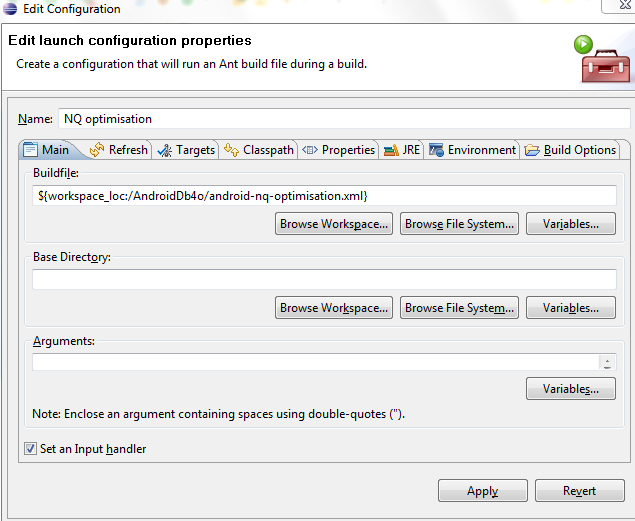
\includegraphics[width=\maxwidth]{images/ref-platform-specific-issues-android-ant-main.png}
\end{center}
Then go to the 'Properties'-tab. There add a new property 'android.platform' which points to the right Android-platform and version-path. You can find the platforms in you Android-SDK. The platforms are in the folder 'platforms' in the Android SDK. For example when your using the API-level 7 the platform is in the folder 'AndroidSDK/platforms/android-7'

\begin{center}
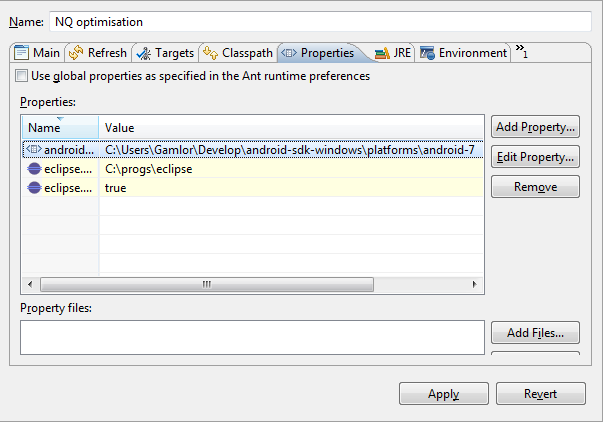
\includegraphics[width=\maxwidth]{images/ref-platform-specific-issues-android-ant-propeties.png}
\end{center}
Apply all settings. The last step is to place the new created builder between the 'Java Builder' and the 'Android Package Builder':

\begin{center}
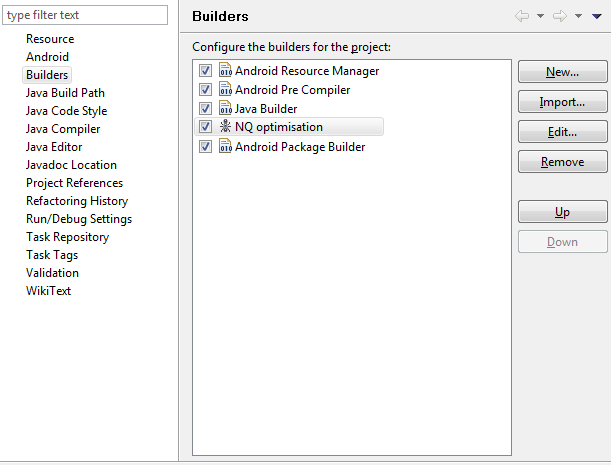
\includegraphics[width=\maxwidth]{images/ref-platform-specific-issues-android-builders.png}
\end{center}
\subsubsection*{Integrating in the Regular Build}

You simply can include the enhancer step into the regular Android build. For that include the enhancer Ant script in the build.xml and let it run during the compilation phase:

\begin{lstlisting}
<import file="${sdk.dir}/tools/ant/build.xml" />

<!-- Add the db4o step below the predefined android targets -->
<import file="android-db4o-optimisation.xml" />

<target name="-post-compile" depends="enhance">
</target>
\end{lstlisting}

{\small\itshape build.xml: Run the enhancer step during the build\par}
\medskip

\subsection{Comparison With SQLite}
\label{ref:platform-specific-issues-android-comparison-with-sqlite}

\href{http://code.google.com/android/}{Android} is a new complete, open and free mobile platform. Android offers developers a Java based software developer kit with lots of helpful APIs, including geolocational services. Of course, there is a database support as well: Android has a built-in support for SQLite database. The basic API is similar to standard JDBC API, with some additional helpful methods\newline{}

It may look better than SQL, but if you look closer it still has the same issues. Queries are specified as strings, so we still stay with a problem of run-time checking instead of compile-time. Furthermore you still need to map between your object-model and the relational SQLite database.

Luckily even for this very early Android release we already have an alternative - db4o. db4o runs on Android out of the box and produces very competitive results as well. The following examples compare db4o and SQLite usage for basic operations.

\begin{itemize}
\item \hyperref[ref:platform-specific-issues-android-general-info]{General Info} (p.~\pageref{ref:platform-specific-issues-android-general-info})
\item \hyperref[ref:platform-specific-issues-android-opening-a-database]{Opening A Database} (p.~\pageref{ref:platform-specific-issues-android-opening-a-database})
\item \hyperref[ref:platform-specific-issues-android-storing-data]{Storing Data} (p.~\pageref{ref:platform-specific-issues-android-storing-data})
\item \hyperref[ref:platform-specific-issues-android-retrieving-data]{Retrieving Data} (p.~\pageref{ref:platform-specific-issues-android-retrieving-data})
\item \hyperref[ref:platform-specific-issues-android-changing-data]{Changing Data} (p.~\pageref{ref:platform-specific-issues-android-changing-data})
\item \hyperref[ref:platform-specific-issues-android-deleting-data]{Deleting Data} (p.~\pageref{ref:platform-specific-issues-android-deleting-data})
\item \hyperref[ref:platform-specific-issues-android-backup]{Backup} (p.~\pageref{ref:platform-specific-issues-android-backup})
\item \hyperref[ref:platform-specific-issues-android-closing-a-database]{Closing A Database} (p.~\pageref{ref:platform-specific-issues-android-closing-a-database})
\item \hyperref[ref:platform-specific-issues-android-schema-evolution]{Schema Evolution} (p.~\pageref{ref:platform-specific-issues-android-schema-evolution})
\end{itemize}

\subsubsection{General Info}
\label{ref:platform-specific-issues-android-general-info}

Both db4o and SQLite are embedded databases, i.e. they run within an application process, removing the overhead associated with a client-server configuration, although db4o can also be used in client-server mode. Both db4o and SQLite offer zero-configuration run modes, which allows to get the database up and running immediately.

\paragraph*{Access Control}

SQLite relies solely on the file system for its database permissions and has no concept of user accounts. SQLite has database-level locks and does not support client/server mode.

db4o can use encryption or client/server mode for user access control. Client/server can also be used in embedded mode, i.e on the same device.

\paragraph*{Referential Integrity}

Traditionally referential integrity in relational databases is implemented with the help of foreign keys. However SQLite \href{http://www.sqlite.org/omitted.htm}{does not support} this feature. In db4o referential integrity is imposed by the object model, i.e. you can't reference an object that does not exist.

\paragraph*{Transactions}

Both db4o and SQLite support ACID transactions.

In db4o all the work is transactional: transaction is implicitly started when the database is open and closed either by explicit commit() call or by close() call through implicit commit. Data is protected from system crash during all application lifecycle. If a crash occurs during commit itself, the commit will be restarted when the system is up again if the system had enough time to write the list of changes, otherwise the transaction will be rolled back to the last safe state.

In SQLite autocommit feature is used by default: transaction is started when a SQL command other than SELECT is executed and commit is executed as soon as pending operation is finished. Explicit BEGIN and END TRANSACTION(COMMIT) or ROLLBACK can be used alternatively to specify user-defined transaction limits. Database crash always results in pending transaction rollback. Nested transactions are not supported.

\paragraph*{Database Size}

Though embeddable db4o and SQLite support big database files:

\begin{itemize}
\item db4o up to 256 GB
\item SQLite up to 2TB
\end{itemize}

all the data is stored in a single database file. db4o also supports clustered databases.

\subsubsection{Opening a Database}
\label{ref:platform-specific-issues-android-opening-a-database}

Opening the database is very similar.

\paragraph*{SQLite}

Opening a SQLite database is very easy. However is necessary to generate the schema for the database.

\begin{lstlisting}
SQLiteDatabase db = _context.openOrCreateDatabase(DATABASE_NAME,
        Context.MODE_PRIVATE, null);
\end{lstlisting}

{\small\itshape SqlExample.java: opening SQLite database\par}
\medskip

\begin{lstlisting}
db.execSQL("CREATE TABLE IF NOT EXISTS " + DB_TABLE_PILOT + " ("
        + "id INTEGER PRIMARY KEY AUTOINCREMENT, "
        + "name TEXT NOT NULL, points INTEGER NOT NULL);");
// Foreign key constraint is parsed but not enforced
// Here it is used for documentation purposes
db.execSQL("CREATE TABLE IF NOT EXISTS " + DB_TABLE_CAR + " ("
        + "id INTEGER PRIMARY KEY AUTOINCREMENT, "
        + "model TEXT NOT NULL, pilot INTEGER NOT NULL,"
        + "FOREIGN KEY (pilot)"
        + "REFERENCES pilot(id) ON DELETE CASCADE);");
db.execSQL("CREATE INDEX IF NOT EXISTS CAR_PILOT ON " + DB_TABLE_CAR
        + " (pilot);");
\end{lstlisting}

{\small\itshape SqlExample.java: SQLite create the schema\par}
\medskip

\paragraph*{db4o}

Opening a db4o database is easy. First you need to create a file which is in the context of the application. Then you can open the database. To be faster, we configure additional indexes.

\begin{lstlisting}
String filePath = context.getFilesDir() + "/android.db4o";
ObjectContainer db = Db4oEmbedded.openFile(configure(), filePath);
\end{lstlisting}

{\small\itshape Db4oExample.java: open a db4o database\par}
\medskip

\begin{lstlisting}
EmbeddedConfiguration configuration = Db4oEmbedded.newConfiguration();
      configuration.common().add(new AndroidSupport());
configuration.common().objectClass(Car.class).objectField("pilot").indexed(true);
configuration.common().objectClass(Pilot.class).objectField("points").indexed(true);
\end{lstlisting}

{\small\itshape Db4oExample.java: configure db4o\par}
\medskip

\paragraph*{Conclusion}

db4o code is a bit more compact, but the main advantage of db4o is in the fact that all APIs are pure java, they are compile-time checked and can be transferred into IDE templates (database opening should be a template as it most probably be the same for all your db4o applications including tests).

\subsubsection{Storing Data}
\label{ref:platform-specific-issues-android-storing-data}

Storing a car-object in is very-different in SQLite and db4o.

\paragraph*{SQLite}

\begin{lstlisting}
ContentValues initialValues = new ContentValues();

initialValues.put("id", number);
initialValues.put("name", "Tester");
initialValues.put("points", number);
db.insert(DB_TABLE_PILOT, null, initialValues);

initialValues = new ContentValues();

initialValues.put("model", "BMW");
initialValues.put("pilot", number);
db.insert(DB_TABLE_CAR, null, initialValues);
\end{lstlisting}

{\small\itshape SqlExample.java: store a car in SQLite\par}
\medskip

\paragraph*{db4o}

\begin{lstlisting}
Car car = new Car("BMW");
car.setPilot(new Pilot("Tester", points));
container.store(car);
\end{lstlisting}

{\small\itshape Db4oExample.java: store a car in db4o\par}
\medskip

\paragraph*{Conclusion}

You can see that db4o handles adding objects to the database in a much more elegant way - \#store(object) method is enough. In SQLite case it is much more difficult as you mush store different objects into different tables. Some of the additional work that SQLite developer will have to do is not visible in this example, i.e:

\begin{itemize}
\item the developer will have to ensure that the sequence of insert commands starts from children objects and goes up to the parent (this can be a really difficult task for relational models including lots of foreign key dependencies);
\item in most cases the data for insertion will come from business objects, which will mean that the object model will have to be transferred to relational model.
\end{itemize}

\subsubsection{Retrieving Data}
\label{ref:platform-specific-issues-android-retrieving-data}

In order to test the retrieval abilities of both databases we will try to select a car with a pilot having15 points:

\paragraph*{SQLite}

\begin{lstlisting}
SQLiteDatabase db = database();
Cursor cursor = db.rawQuery(
        "SELECT c.model, p.name, p.points, r.id, r.year" + " FROM "
                + DB_TABLE_CAR + " c, " + DB_TABLE_PILOT + " p "
                + "WHERE c.pilot = p.id AND p.points = ?;",
        new String[] { "15" });
cursor.moveToFirst();

Pilot pilot = new Pilot();
pilot.setName(cursor.getString(1));
pilot.setPoints(cursor.getInt(2));

Car car = new Car();
car.setModel(cursor.getString(0));
car.setPilot(pilot);
\end{lstlisting}

{\small\itshape SqlExample.java: select a car from SQLite\par}
\medskip

\paragraph*{db4o}

\begin{lstlisting}
ObjectContainer db = database();
ObjectSet<Car> cars = db.query(new Predicate<Car>() {
    @Override
    public boolean match(Car car) {
        return car.getPilot().getPoints() == 15;
    }
});

Car car = cars.get(0);
\end{lstlisting}

{\small\itshape Db4oExample.java: select a car from db4o\par}
\medskip

\paragraph*{Conclusion}

The db4o native queries are typesafe. This is a huge benefit, since the compiler can detect errors and the IDE help you with the refactoring. In the example above you can see that SQLite needs a lot of additional code to transfer the retrieved data into application's objects, whereas db4o does not need this code at all, as the result is already a collection of objects.

\subsubsection{Changing Data}
\label{ref:platform-specific-issues-android-changing-data}

For this test we will select and update a car with a new pilot, where existing pilot has 15 points:

\paragraph*{SQLite}

\begin{lstlisting}
SQLiteDatabase db = database();
db.execSQL("INSERT INTO REG_RECORDS (id,year) VALUES ('A1', DATETIME('NOW'))");

ContentValues updateValues = new ContentValues();
updateValues.put("reg_record", "A1");
int count = db.update(DB_TABLE_CAR, updateValues,
        "pilot IN (SELECT id FROM " + DB_TABLE_PILOT
                + " WHERE points = 15)", null);
if (count == 0) {
    logToConsole(0, "Car not found, refill the database to continue.",
            false);
} else {
    Cursor c = db.rawQuery("SELECT c.model, r.id, r.year from car c, "
            + "REG_RECORDS r, pilot p where c.reg_record = r.id "
            + "AND c.pilot = p.id AND p.points = 15;", null);
    if (c.getCount() == 0) {
        logToConsole(0,
                "Car not found, refill the database to continue.",
                false);
        return;
    }
    c.moveToFirst();
    String date = c.getString(2);
    
    Date dt = parseDate(date);
    RegistrationRecord record = new RegistrationRecord(c.getString(1),dt);
    
    Car car = new Car();
    car.setModel(c.getString(0));
    car.setRegistration(record);
    logToConsole(startTime, "Updated Car (" + car + "): ", true);
}
\end{lstlisting}

{\small\itshape SqlExample.java: update a car with SQLite\par}
\medskip

\paragraph*{db4o}

\begin{lstlisting}
ObjectContainer container = database();
if (container != null){
    ObjectSet<Car>  result = container.query(new Predicate<Car>(){
        @Override
        public boolean match(Car car) {
            return car.getPilot().getPoints()==15;
        }
        
    });
    if (!result.hasNext()){
        logToConsole(0, "Car not found, refill the database to continue.", false);
    } else {
        Car car = result.next();
        logToConsole(startTime, "Selected Car (" + car + "): ", false);
        startTime = System.currentTimeMillis();
        car.setRegistration(new RegistrationRecord("A1", new Date()));
        logToConsole(startTime, "Updated Car (" + car + "): ", true);
    }            
}
\end{lstlisting}

{\small\itshape Db4oExample.java: update a car with db4o\par}
\medskip

\paragraph*{Conclusion}

In this example db4o and SQLite actually behave quite differently. For SQLite in order to update a pilot in an existing car in the database the following actions are needed:

\begin{enumerate}
\item A new pilot should be created and saved to the database.
\item New pilot's primary key (101) should be retrieved (not shown in this example, but is necessary for a real database application).
\item An update statement should be issued to replace pilot field in the car table.
\end{enumerate}

For db4o database the sequence will be the following:

\begin{enumerate}
\item Retrieve the car from the database
\item Update the car with a new pilot object
\end{enumerate}

As you can see the only benefit of SQLite API is that the car can be selected and updated in one statement. But in the same time there are serious disadvantages:

\begin{itemize}
\item A new pilot record should be created absolutely separately (in a real database will also include ORM)
\item The pilot's ID needs to be retrieved separately (we must sure that it is a correct id)
\end{itemize}

In db4o we avoid these disadvantages as creating new pilot and updating the car value are actually combined in one atomic operation.

\subsubsection{Deleting Data}
\label{ref:platform-specific-issues-android-deleting-data}

The following methods will delete a car with a pilot having 5 points from each database:

\paragraph*{SQLite}

\begin{lstlisting}
SQLiteDatabase db = database();
db.delete(DB_TABLE_CAR,
        "pilot in (select id from pilot where points = ?)",
        new String[]{"5"});
\end{lstlisting}

{\small\itshape SqlExample.java: delete a car with SQLite\par}
\medskip

\paragraph*{db4o}

\begin{lstlisting}
ObjectContainer db = database();
ObjectSet<Car> cars = db.query(new Predicate<Car>() {
    public boolean match(Car car) {
        return car.getPilot().getPoints()==5;
    }            
});
for(Car car : cars){
    db.delete(car);
}
\end{lstlisting}

{\small\itshape Db4oExample.java: delete a car with db4o\par}
\medskip

\paragraph*{Conclusion}

In this example db4o code looks much longer. But should we consider it a disadvantage? My opinion is - No. Of course, SQLite seems to handle the whole operation in just one statement: db.delete(). But if you look attentively you will see that basically this statement just transfers all the difficult job to SQL: SQL statement should select a pilot with a given condition, then find a car. Using SQL can look shorter but it has a great disadvantage - it uses strings. So what will happen if the statement is wrong? You will never notice it till somebody in the running application will cause this statement to execute. Even then you might not see the reason immediately. The same applies to the schema changes - you may not even notice that you are using wrong tables and fields.

db4o helps to avoid all the above mentioned problems: query syntax is completely compile-checked and schema evolution will be spotted immediately by the compiler, so that you would not need to rely on code search and replace tools.

\subsubsection{Backup}
\label{ref:platform-specific-issues-android-backup}

\paragraph*{SQLite}

SQLite does not support a special API to make a backup. However, as you remember SQLite database is stored in a single database file, so the backup can be simply a matter of copying the database file. Unfortunately, this can't be done if the database is in use. In this case you can use \href{http://code.google.com/android/reference/adb.htm}{Android Debug Bridge} (adb) tool to access sqlite3 command-line application, which has .dump command for backing up database contents while the database is in use:

\begin{lstlisting}
E:\>adb shell
# sqlite3 /data/data/com.db4odoc.android.compare/databases/android.db
sqlite3 /data/data/com.db4odoc.android.compare/databases/android.db
SQLite version 3.5.0
Enter ".help" for instructions
sqlite> .dump > android200711.dmp
.dump > android200711.dmp
BEGIN TRANSACTION;
COMMIT;
sqlite>.exit
.exit
# ^D
\end{lstlisting}

Ctrl+D command is used to close adb session.

\paragraph*{db4o}

On db4o a ExtObjectContainer\#backup call is used to backup a database in use. \hyperref[ref:advanced-topics-backup]{See "Backup"} (p.~\pageref{ref:advanced-topics-backup})

\subsubsection{Closing a Database}
\label{ref:platform-specific-issues-android-closing-a-database}

The following methods will close SQLite and db4o database accordingly:

\paragraph*{SQLite}

\begin{lstlisting}
_db.close();
\end{lstlisting}

{\small\itshape SqlExample.java: close SQLite\par}
\medskip

\paragraph*{db4o}

\begin{lstlisting}
container.close();
\end{lstlisting}

{\small\itshape Db4oExample.java: close db4o\par}
\medskip

\subsubsection{Schema Evolution}
\label{ref:platform-specific-issues-android-schema-evolution}

When a new application development is considered it is important to think about its evolution. What happens if your initial model does not suffice and you need changes or additions? Let's look how db4o and SQLite applications can handle it.

To keep the example simple, let's add a registration record to our car:

\begin{lstlisting}
private RegistrationRecord registration;
   
public RegistrationRecord getRegistration() {
    return registration;
}

public void setRegistration(RegistrationRecord registration) {
    this.registration = registration;
}
\end{lstlisting}

{\small\itshape Car.java: Add a new field to the car\par}
\medskip

Ok, the application is changed to take care for the new class. What about our databases?

\subparagraph*{Schema Evolution in db4o}

db4o supports such schema change on the fly: we can select values and update the new field too:

\begin{lstlisting}
ObjectContainer container = database();
if (container != null){
    ObjectSet<Car>  result = container.query(new Predicate<Car>(){
        @Override
        public boolean match(Car car) {
            return car.getPilot().getPoints()==15;
        }
        
    });
    if (!result.hasNext()){
        logToConsole(0, "Car not found, refill the database to continue.", false);
    } else {
        Car car = result.next();
        logToConsole(startTime, "Selected Car (" + car + "): ", false);
        startTime = System.currentTimeMillis();
        car.setRegistration(new RegistrationRecord("A1", new Date()));
        logToConsole(startTime, "Updated Car (" + car + "): ", true);
    }            
}
\end{lstlisting}

{\small\itshape Db4oExample.java: update a car with db4o\par}
\medskip

\subparagraph*{Schema Evolution in SQLite}

For SQLite database model should be synchronized with the object model:

\begin{lstlisting}
db.execSQL("CREATE TABLE IF NOT EXISTS REG_RECORDS ("
        + "id TEXT PRIMARY KEY, year DATE);");
db.execSQL("CREATE INDEX  IF NOT EXISTS  IDX_REG_RECORDS ON REG_RECORDS (id);");
db.execSQL("ALTER TABLE " + DB_TABLE_CAR + " ADD reg_record TEXT;");
\end{lstlisting}

{\small\itshape SqlExample.java: upgrade schema in SQLite\par}
\medskip

Now we can try to retrieve and update records:

\begin{lstlisting}
SQLiteDatabase db = database();
db.execSQL("INSERT INTO REG_RECORDS (id,year) VALUES ('A1', DATETIME('NOW'))");

ContentValues updateValues = new ContentValues();
updateValues.put("reg_record", "A1");
int count = db.update(DB_TABLE_CAR, updateValues,
        "pilot IN (SELECT id FROM " + DB_TABLE_PILOT
                + " WHERE points = 15)", null);
if (count == 0) {
    logToConsole(0, "Car not found, refill the database to continue.",
            false);
} else {
    Cursor c = db.rawQuery("SELECT c.model, r.id, r.year from car c, "
            + "REG_RECORDS r, pilot p where c.reg_record = r.id "
            + "AND c.pilot = p.id AND p.points = 15;", null);
    if (c.getCount() == 0) {
        logToConsole(0,
                "Car not found, refill the database to continue.",
                false);
        return;
    }
    c.moveToFirst();
    String date = c.getString(2);
    
    Date dt = parseDate(date);
    RegistrationRecord record = new RegistrationRecord(c.getString(1),dt);
    
    Car car = new Car();
    car.setModel(c.getString(0));
    car.setRegistration(record);
    logToConsole(startTime, "Updated Car (" + car + "): ", true);
}
\end{lstlisting}

{\small\itshape SqlExample.java: update a car with SQLite\par}
\medskip

\subparagraph*{Conclusion}

You can see that schema evolution is much easier with db4o. But the main difficulty that is not visible from the example is that schema evolution with SQLite database can potentially introduce a lot of bugs that will be difficult to spot. For more information see \hyperref[ref:advanced-topics-refactoring-and-schema-evolution]{Refactoring and Schema Evolution} (p.~\pageref{ref:advanced-topics-refactoring-and-schema-evolution}).

\subsection{Proguard}
\label{ref:platform-specific-issues-android-proguard}

The Android SDK includes Proguard to shrink the size of the application by removing unused stuff, shorting names and other optimisations.

db4o relies heavily on reflection, which can lead to major issues when code is processed with Proguard. db4o has not been tested under such a environment. When you're using Proguard you need to test yourself if your application is still working.

You should to exclude all persisted classes from the shrinking process, because db4o manages objects by their name. Therefore db4o will have issue when those name changes by the shrinking process. Read the \href{http://proguard.sourceforge.net/index.html\#/manual/usage.html}{Proguard documentation} for the right configuration. For example when your persisted classes in a certain package you can exclude them like this:

\begin{lstlisting}
########################
-keep class com.db4odoc.android.**
-keepnames class com.db4odoc.android.**
-keepclassmembers class com.db4odoc.android.** {
    !static !transient <fields>;
    !private <fields>;
    !private <methods>;
}
\end{lstlisting}

{\small\itshape proguard.cfg: Keep persisted classes intact\par}
\medskip

To be on the save side you should keep all db4o classes in the original state. Especially since db4o stores some internal data structures which shouldn't be renamed.

\begin{lstlisting}
########################
## Monitoring requires JMX, which is not available on Android
-dontwarn com.db4o.monitoring.*
-dontwarn com.db4o.cs.monitoring.*
-dontwarn com.db4o.internal.monitoring.*

## Ant is usually not used in a running app
-dontwarn com.db4o.instrumentation.ant.*
-dontwarn com.db4o.ta.instrumentation.ant.*

## Keep internal classes.
-keep class com.db4o.** { *; }
\end{lstlisting}

{\small\itshape proguard.cfg: keep db4o intact\par}
\medskip

\section{db4o On Java Platforms}
\label{ref:platform-specific-issues-db4o-on-java-platforms}

\subsection*{All Java}

\begin{itemize}
\item root package is com.db4o
\end{itemize}

\subsection*{JDK 1.5 or newer}

\begin{itemize}
\item Generics support introduced in JDK1.5 makes db4o Native Query syntax much simpler: \texttt{List \textless{}Pilot\textgreater{} pilots = db.query(new Predicate \textless{}Pilot\textgreater{} () \{ public boolean match(Pilot pilot) \{ return pilot.getPoints() == 100;\}\});}
\item following JDK5 annotations db4o introduces its own annotations.
\item you can use built-in enums
\item db4o for JDK5 also has replication support.
\end{itemize}

\subsection*{Android}

Read about how to use \hyperref[ref:platform-specific-issues-android]{db4o on Android here} (p.~\pageref{ref:platform-specific-issues-android}).

\section{Security Requirements On Java Platform}
\label{ref:platform-specific-issues-security-requirements-on-java-platform}

Java Security Manager can be used to specify Java application security permissions. It is usually provided by web-browsers and web-servers for applet and servlet execution, however any Java application can make use of a security manager. For example, to use the default security manager you will only need to pass \texttt{-Djava.security.manager} option to JVM command line. Custom security managers can be created and utilized as well (please refer to Java documentation for more information).

If you are going to use db4o in a Tomcat servlet container you will need to grant some additional permissions in \{CATALINA\_HOME\}/conf/catalina.policy file:

\begin{lstlisting}
// The permissions granted to the context 
WEB-INF/classes directory 
grant codeBase "file:${catalina.home}/webapps/{your_db4o_application}/WEB-INF/classes/-" 
{ 
    permission java.util.PropertyPermission "user.home", "read"; 
    permission java.util.PropertyPermission "java.fullversion", "read";    
    permission java.io.FilePermission "path_to_db4o_database_folder", "read";    
    permission java.io.FilePermission "path_to_db4o_database_file", "read, write"; 
}; 
// The permissions granted to the context WEB-INF/lib directory, containing db4o jar 
grant codeBase "file:${catalina.home}/webapps/{your_db4o_application}/WEB-INF/lib/-" 
{    
    permission java.io.FilePermission "path_to_db4o_database_file", "read, write"; 
};
            
\end{lstlisting}

An example catalina.policy file:

\begin{lstlisting}
// Licensed to the Apache Software Foundation (ASF) under one or more
// contributor license agreements.  See the NOTICE file distributed with
// this work for additional information regarding copyright ownership.
// The ASF licenses this file to You under the Apache License, Version 2.0
// (the "License"); you may not use this file except in compliance with
// the License.  You may obtain a copy of the License at
//
//     http://www.apache.org/licenses/LICENSE-2.0
//
// Unless required by applicable law or agreed to in writing, software
// distributed under the License is distributed on an "AS IS" BASIS,
// WITHOUT WARRANTIES OR CONDITIONS OF ANY KIND, either express or implied.
// See the License for the specific language governing permissions and
// limitations under the License.

// ============================================================================
// catalina.corepolicy - Security Policy Permissions for Tomcat 6
//
// This file contains a default set of security policies to be enforced (by the
// JVM) when Catalina is executed with the "-security" option.  In addition
// to the permissions granted here, the following additional permissions are
// granted to the codebase specific to each web application:
//
// * Read access to the document root directory
//
// $Id: catalina.policy 609294 2008-01-06 11:43:46Z markt $
// ============================================================================

// ========== SYSTEM CODE PERMISSIONS =========================================

// These permissions apply to javac
grant codeBase "file:${java.home}/lib/-" {
        permission java.security.AllPermission;
};

// These permissions apply to all shared system extensions
grant codeBase "file:${java.home}/jre/lib/ext/-" {
        permission java.security.AllPermission;
};

// These permissions apply to javac when ${java.home] points at $JAVA_HOME/jre
grant codeBase "file:${java.home}/../lib/-" {
        permission java.security.AllPermission;
};

// These permissions apply to all shared system extensions when
// ${java.home} points at $JAVA_HOME/jre
grant codeBase "file:${java.home}/lib/ext/-" {
        permission java.security.AllPermission;
};

// ========== CATALINA CODE PERMISSIONS =======================================

// These permissions apply to the daemon code
grant codeBase "file:${catalina.home}/bin/commons-daemon.jar" {
        permission java.security.AllPermission;
};

// These permissions apply to the logging API
grant codeBase "file:${catalina.home}/bin/tomcat-juli.jar" {
        permission java.security.AllPermission;

        permission java.util.PropertyPermission "java.util.logging.config.class", "read";
        permission java.util.PropertyPermission "java.util.logging.config.file", "read";
        permission java.lang.RuntimePermission "shutdownHooks";
        permission java.io.FilePermission "${catalina.base}${file.separator}conf${file.separator}logging.properties", "read";
        permission java.util.PropertyPermission "catalina.base", "read";
        permission java.util.logging.LoggingPermission "control";
        permission java.io.FilePermission "${catalina.base}${file.separator}logs", "read, write";
        permission java.io.FilePermission "${catalina.base}${file.separator}logs${file.separator}*", "read, write";
        permission java.lang.RuntimePermission "getClassLoader";
        // To enable per context logging configuration, permit read access to the appropriate file.
        // Be sure that the logging configuration is secure before enabling such access
        // eg for the examples web application:
        // permission java.io.FilePermission "${catalina.base}${file.separator}webapps${file.separator}examples${file.separator}WEB-INF${file.separator}classes${file.separator}logging.properties", "read";
};

// These permissions apply to the server startup code
grant codeBase "file:${catalina.home}/bin/bootstrap.jar" {
        permission java.security.AllPermission;
};

// These permissions apply to the servlet API classes
// and those that are shared across all class loaders
// located in the "lib" directory
grant codeBase "file:${catalina.home}/lib/-" {
        permission java.security.AllPermission;
};

// ========== WEB APPLICATION PERMISSIONS =====================================

// These permissions are granted by default to all web applications
// In addition, a web application will be given a read FilePermission
// and JndiPermission for all files and directories in its document root.
grant { 
    // Required for JNDI lookup of named JDBC DataSource's and
    // javamail named MimePart DataSource used to send mail
    permission java.util.PropertyPermission "java.home", "read";
    permission java.util.PropertyPermission "java.naming.*", "read";
    permission java.util.PropertyPermission "javax.sql.*", "read";

    // OS Specific properties to allow read access
    permission java.util.PropertyPermission "os.name", "read";
    permission java.util.PropertyPermission "os.version", "read";
    permission java.util.PropertyPermission "os.arch", "read";
    permission java.util.PropertyPermission "file.separator", "read";
    permission java.util.PropertyPermission "path.separator", "read";
    permission java.util.PropertyPermission "line.separator", "read";

    // JVM properties to allow read access
    permission java.util.PropertyPermission "java.version", "read";
    permission java.util.PropertyPermission "java.vendor", "read";
    permission java.util.PropertyPermission "java.vendor.url", "read";
    permission java.util.PropertyPermission "java.class.version", "read";
    permission java.util.PropertyPermission "java.specification.version", "read";
    permission java.util.PropertyPermission "java.specification.vendor", "read";
    permission java.util.PropertyPermission "java.specification.name", "read";

    permission java.util.PropertyPermission "java.vm.specification.version", "read";
    permission java.util.PropertyPermission "java.vm.specification.vendor", "read";
    permission java.util.PropertyPermission "java.vm.specification.name", "read";
    permission java.util.PropertyPermission "java.vm.version", "read";
    permission java.util.PropertyPermission "java.vm.vendor", "read";
    permission java.util.PropertyPermission "java.vm.name", "read";

    // Required for OpenJMX
    permission java.lang.RuntimePermission "getAttribute";

    // Allow read of JAXP compliant XML parser debug
    permission java.util.PropertyPermission "jaxp.debug", "read";

    // Precompiled JSPs need access to this package.
    permission java.lang.RuntimePermission "accessClassInPackage.org.apache.jasper.runtime";
    permission java.lang.RuntimePermission "accessClassInPackage.org.apache.jasper.runtime.*";
    
    // Precompiled JSPs need access to this system property.
    permission java.util.PropertyPermission "org.apache.jasper.runtime.BodyContentImpl.LIMIT_BUFFER", "read";

};

// The permissions granted to the context WEB-INF/classes directory
grant codeBase "file:${catalina.home}/webapps/Db4oSite/WEB-INF/classes/-" {
   permission java.util.PropertyPermission "user.home", "read";  
   permission java.util.PropertyPermission "java.fullversion", "read";
   permission java.io.FilePermission "${user.home}${file.separator}db4o${file.separator}data", "read";
   permission java.io.FilePermission "${user.home}${file.separator}db4o${file.separator}data${file.separator}test.db4o.yap", "read, write";
};

grant codeBase "file:${catalina.home}/webapps/Db4oSite/WEB-INF/lib/-" {
   permission java.io.FilePermission "${user.home}${file.separator}db4o${file.separator}data${file.separator}test.db4o.yap", "read, write";
};

// You can assign additional permissions to particular web applications by
// adding additional "grant" entries here, based on the code base for that
// application, /WEB-INF/classes/, or /WEB-INF/lib/ jar files.
//
// Different permissions can be granted to JSP pages, classes loaded from
// the /WEB-INF/classes/ directory, all jar files in the /WEB-INF/lib/
// directory, or even to individual jar files in the /WEB-INF/lib/ directory.
//
// For instance, assume that the standard "examples" application
// included a JDBC driver that needed to establish a network connection to the
// corresponding database and used the scrape taglib to get the weather from
// the NOAA web server.  You might create a "grant" entries like this:
//
// The permissions granted to the context root directory apply to JSP pages.
// grant codeBase "file:${catalina.home}/webapps/examples/-" {
//      permission java.net.SocketPermission "dbhost.mycompany.com:5432", "connect";
//      permission java.net.SocketPermission "*.noaa.gov:80", "connect";
// };
//
// The permissions granted to the context WEB-INF/classes directory
// grant codeBase "file:${catalina.home}/webapps/examples/WEB-INF/classes/-" {
// };
//
// The permission granted to your JDBC driver
// grant codeBase "jar:file:${catalina.home}/webapps/examples/WEB-INF/lib/driver.jar!/-" {
//      permission java.net.SocketPermission "dbhost.mycompany.com:5432", "connect";
// };
// The permission granted to the scrape taglib
// grant codeBase "jar:file:${catalina.home}/webapps/examples/WEB-INF/lib/scrape.jar!/-" {
//      permission java.net.SocketPermission "*.noaa.gov:80", "connect";
// };
\end{lstlisting}

In order to avoid db4o DatabaseFileLocked exception you will also need to add some configuration before opening the object container:\newline{}

\texttt{Configuration config = Db4o.newConfiguration();\newline{}}

\texttt{config.lockDatabaseFile(false);\newline{}}

\texttt{ObjectContainer container = Db4o.openFile(config, dbfile.getPath());\newline{}}

Having done that, you can package and deploy your application. To enable the security configuration start Tomcat with the following command:\newline{}

\{CATALINA\_HOME\}/bin/catalina start -security \newline{}

\section{XML Import-Export}
\label{ref:platform-specific-issues-xml-import-export}

One of the most widely used platform independent formats of data exchange today is xml.

db4o does not provide any specific API to be used for XML import/export, but with the variety of XML serialization libraries available.

All that you need to export your database/query results is:

\begin{enumerate}
\item Retrieve objects from the database.
\item Serialize them in XML format using your favorite serialization API/library
\item Save XML stream (to a disc location, into memory, into another database).
\end{enumerate}

Import process is just the reverse:

\begin{enumerate}
\item Read the XML stream.
\item Create an objects from XML.
\item Save objects to db4o.
\end{enumerate}

Let's go through a simple example. We will use XStream library (\href{http://xstream.codehaus.org/}{http://xstream.codehaus.org/}) for object serialization, but any other tool capable of serializing objects into XML will do as well.

\begin{lstlisting}
ObjectContainer container = Db4oEmbedded.openFile("database.db4o");
try {
    Pilot[] pilots = container.query(Pilot.class).toArray(new Pilot[0]);
    XStream xstream = new XStream();
    OutputStream stream = new FileOutputStream("pilots.xml");
    try {
        xstream.toXML(pilots, stream);
    } finally {
        stream.close();
    }
} finally {
    container.close();
}
\end{lstlisting}

{\small\itshape XMLSerialisationExamples.java: Serialize to XML\par}
\medskip

After the method executes all car objects from the database will be stored in the export file as an array. Note that child objects (Pilot) are stored as well without any additional settings. You can check the created XML file to see how it looks like.

Now we can clean the database and try to recreate it from the XML file:

\begin{lstlisting}
ObjectContainer container = Db4oEmbedded.openFile("database.db4o");
try {
    XStream xstream = new XStream();
    InputStream stream = new FileInputStream("pilots.xml");
    try {
        Pilot[] pilots = (Pilot[]) xstream.fromXML(stream);
        for (Pilot pilot : pilots) {
            container.store(pilot);
        }
    } finally {
        stream.close();
    }
} finally {
    container.close();
}
\end{lstlisting}

{\small\itshape XMLSerialisationExamples.java: Read objects from XML\par}
\medskip

Obviously there is much more to XML serialization: renaming fields, storing collections, selective persistence etc. You should be able to find detailed description together with the serialization library, which you will use.

\section{OSGi}
\label{ref:platform-specific-issues-database-for-osgi}

db4o can run in an OSGi environment. db4o jars have a OSGi manifest so that you can use them in your project.

\subsection*{Using db4o with OSGi}

In principal you can use db4o in OSGi without any special configuration, as long as the stored objects and db4o are loaded with the same OSGi classloader.

However as soon as you're using multiple bundles, and therefore multiple classloaders, you need to configure db4o. You can \hyperref[ref:configuration-common-reflector]{specify the class-loader explicitly} (p.~\pageref{ref:configuration-common-reflector}) for db4o, or even use multiple class-loaders. This way you can lookup in multiple class-loaders for your class. First write an implementation of the JdkLoader interface:

\begin{lstlisting}
class OSGiLoader implements JdkLoader{
    private final Bundle[] bundlesToLookIn;

    OSGiLoader(Bundle... bundlesToLookIn) {
        this.bundlesToLookIn = bundlesToLookIn;
    }

    public Class loadClass(String s) {
        for (Bundle bundle : bundlesToLookIn) {
            try {
                return bundle.loadClass(s);
            } catch (ClassNotFoundException e) {
                // just retry on other bundles
            }
        }
        try {
            return getClass().getClassLoader().loadClass(s);
        } catch (ClassNotFoundException e) {
            return null;
        }
    }

    public Object deepClone(Object o) {
        return new OSGiLoader(bundlesToLookIn);
    }
}
\end{lstlisting}

{\small\itshape UsingDb4oDirectly.java: Load classes from multiple bundles\par}
\medskip

After that you can use your implementation to load classes for db4o:

\begin{lstlisting}
// Specify the bundles from which the classes are used to store objects
Bundle[] bundles = new Bundle[]{bundleContext.getBundle()};
EmbeddedConfiguration configuration = Db4oEmbedded.newConfiguration();
configuration.common()
        .reflectWith(new JdkReflector(new OSGiLoader(bundles)));
\end{lstlisting}

{\small\itshape UsingDb4oDirectly.java: Db4o with a special OSGi loader\par}
\medskip

Note also that some db4o jars have a dependency on Ant and need an Ant bundle in your OSGi application to use all features.

\subsection*{Using the db4o OSGi package}

An alternative is to use the db4o OSGi package, which is in the db4o--X.XX-osgi.jar and includes all dependencies. \hyperref[ref:dependency-overview]{See "Dependency Overview"} (p.~\pageref{ref:dependency-overview}). This provides a OSGi service which creates a db4o instance for you. It configures db4o in such a way that classes are loaded from the requesting OSGi service.

\begin{lstlisting}
ServiceReference reference = bundleContext.getServiceReference("com.db4o.osgi.Db4oService");
Db4oService db4oService = (Db4oService) bundleContext.getService(reference);
ObjectContainer container = db4oService.openFile("database.db4o");
\end{lstlisting}

{\small\itshape UsingDb4oViaService.java: Get db4o osgi service\par}
\medskip

